% !TEX root = ./Vorlesungsmitschrift DIFF 2.tex  
\lecture{Do 14.05. 10:15}{}
\begin{satz}\label{funktion_ableiten_mit_hoeheren_abbildungen}
  Sei \( f\maps \underrelate{\vertrelation{\supset}}{\reals^k}{B_{r_1}^{\norm{\cdot}}(a)}\times \underrelate{\vertrelation{\supset}}{\reals^m}{B_{r_2}^{\norm{\cdot}}(b)}\to \reals^m \) eine Abbildung mit \( f(a,b)=0 \), die in \( (a,b) \) differenzierbar sei. Sei zudem \( D_2 f(a,b) \), definiert über
  \begin{equation*}
    \totalderivative-{f}(a,b)=(\underbrace{\partial_1 f(a,b)\, \cdots\,  \partial_k f(a,b)}_{\defines D_1 f(a,b)\in \Mat(m\times k)}\, \underbrace{\partial_{k+1}f(a,b)\, \cdots\, \partial_{k+m}f(a,b)}_{\defines D_2 f(a,b)\in \Mat(m\times m)}),
  \end{equation*}
  invertierbar. Sei zudem \( g\maps B_{r_1}(a)\to \reals^m \) stetig und gelte \( g(B_{r_1}(a))\subset B_{r_2}(b) \) und \( g(a)=b \) und \( f(x,g(x))=0 \) \tforall \( x\in B_{r_1}(a) \). Dann ist \( g \) in \( a \) differenzierbar und es gilt
  \begin{equation*}
    \totalderivative-{g}(a)=-\inverse{\left( D_2f(a,b) \right)}D_1 f(a,b)\in \Mat(m\times k, \reals).
  \end{equation*}
\end{satz}
\begin{proof}
  Es gilt für \( h=(h_1,h_2)\in B_{r_1}(0)\times B_{r_2}(0) \)
  \begin{equation*}
    f(\underbrace{(a,b)+h}_{=(a+h_1,b+h_2)})=0+D_1f(a,b)\matrixmult h_1+D_2 f(a,b)\matrixmult h_2+\underline{R}_{(a,b)}(h)
  \end{equation*}
  mit \( \frac{\underline{R}_{(a,b)}(h)}{\norm{h}}\goesto 0 \) \tforall \( x\in B_{r_1}(a) \) folgt
  \begin{equation*}
    \begin{split}
      0=f(\underbrace{a+h_1}_{\in B_{r_1}(a)},g(a+h_1))=&D_1 f(a,b)\matrixmult h_1\\
      &+D_2 f(a,b)\matrixmult (g(a+h_1)-b)\\
      &+\underline{R}_{(a,b)}(h_1,g(a+h_1)-b)\quad \forall h_1\in B_{r_1}(0).
    \end{split}
  \end{equation*}
  Also
  \begin{equation*}
    \begin{split}
      g(a+h_1)=&g(a)-\inverse{D_2f(a,b)}\matrixmult D_1 f(a,b)\matrixmult h_1\\
      &\underbrace{-\inverse{D_2f(a,b)}\matrixmult \underline{R}_{(a,b)}(h_1,g(a+h_1)-b)}_{\defines \tilde{R_{a,b}^g(h_1)}}\quad \forall h_1\in B_{r_1}(0).
    \end{split}
  \end{equation*}
  Wir sind fertig, wenn wir zeigen können, dass
  \begin{equation*}
    \frac{\tilde{R}_{a,b}^g(h_1)}{\norm{h_1}}\goesto 0 \text{ für }h_1\goesto 0.
  \end{equation*}
  Wegen der Differenzierbarkeit von \( f \) in \( (a,b) \) \texists  \( \tilde{C} \) und \( \delta_1,\delta_2>0 \), \( \delta_i<r_i \), \sd
  \begin{equation*}
    \norm{\underline{R}_{(a,b)}(h_1,h_2)}\leq \tilde{C}(\norm{h_1}+\norm{h_2})\quad \forall h_1\in B_{\delta_1}(0), h_2\in B_{\delta_2}(0),
  \end{equation*}
  also
  \begin{equation*}
    \norm{\underline{R}_{(a,b)}(h_1,g(a+h_1)-b)}\leq \tilde{C}(\norm{h_1}+\norm{g(a+h_1)-b})
  \end{equation*}
  für alle \( h_1 \) \sd \( \norm{h_1}<\delta_1 \) und \( \norm{g(a+h_1)-b}<\delta_2 \). Wegen der Stetigkeit von \( g \) in \( a \) gibt es \( \delta>0 \),\( \delta<\delta_1 \), \( \norm{g(a+h_1)-\underbrace{g(a)}_{=b}}<\delta_2 \) für alle \( h_1\in B_{\delta}(0) \).
\end{proof}
\begin{bemerkungen*}
  \begin{enumerate}
    \item Ist \( f,g \) wie in \thref{funktion_ableiten_mit_hoeheren_abbildungen} und \( f \) überall \emph{stetig} differenzierbar. Ist dann \( D_2 f(a,b) \) invertierbar. So gibt es eine Umgebung \( V_1\times V_2 \) von \( (a,b) \) \sd \( D_2f(x,y) \) invertiertbar ist für alle \( (x,y)\in V_1\times V_2 \) (denn \( (x,y)\mapsto \Det D_2f(x,y) \) ist stetig, da es ein Polynom stetiger Funktionen ist und \( \Det D_2 f(a,b)\neq 0 \)).
    \item Das Beispiel vom letzten Mal ist genau von diesem Typ.
  \end{enumerate}
\end{bemerkungen*}
Umgekehrt kann man eine Funktion \( g \) wie oben durch \enquote{Auflösen der Gleichung \( f(x,g(x))=0 \)} bestimmen (unter gewissen Voraussetzungen):
\begin{satz}[Satz von der impliziten Funktion]\label{satz_von_der_impliziten_funktion}
  Seien \( U_1\subset \reals^k \), \( U_2\subset \reals^m \) offen und \( f\maps U_1\times U_2\to \reals^m \) stetig differenzierbar. Sei \( (a,b) \in U_1\times U_2 \) \sd \( f(a,b)=0 \) und \( D_2f(a,b)\in \Mat(m \times m,\reals) \) invertierbar. Dann gibt es offene Umgebungen \( V_1\subset U_1 \), \( V_2\subset U_2 \) von \( a \) \bzw \( b \) und eine stetige Funktion \( g\maps V_1\to \reals^m \), \( g(V_1)\subset V_2 \), \sd \( f(x,g(x))=0 \) \tforall  \( x\in V_1 \). Ist \( (x,y)\in V_1\times V_2 \) \sd \( f(x,y)=0 \), so ist \( y=g(x) \).
\end{satz}
\begin{bemerkungen*}
  \begin{enumerate}
    \item \label{implizite_funktion_auf_umgebung_stetig_differenzierbar} Aus \ref{funktion_ableiten_mit_hoeheren_abbildungen} und der folgenden Bemerkung folgt, dass \( g \) in einer eventuell verkleinerten Umgebung \( \tilde{V_1}\subset V_1 \) von \( a \) sogar stetig differenzierbar ist und gilt
    \begin{equation*}
      \totalderivative-{g}(x)=-\inverse{D_2 f(x,g(x))}\matrixmult D_1f(x,g(x))\quad \forall x\in \tilde{V_1}
    \end{equation*}
    \item Für den Satz ist wichtig, dass \( U_1\times U_2 \) gegebenenfalls verkleinert wird:
    \begin{figure}[H]
      \centering
      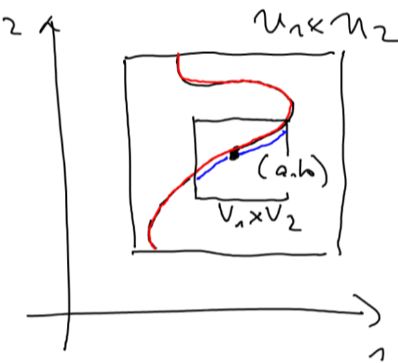
\includegraphics[width=0.5\linewidth]{figures/verkleinerter_definitionsbereich_implizite_funktion}
      \caption*{\textcolor{Blue}{\( \Gamma_g=\Set{(x,g(x))|x\in V_1} \)},\textcolor{Red}{}}
      \label{fig:verkleinerter_definitionsbereich_implizite_funktion}
    \end{figure}
    Betrachtete man auch den oberenTeil der Kurve,könnte man \( x \) nicht ein eindeutiges \( y \) zuordnen.
    \item Die Einschränkung auf Definitionsbeiche der Form \( U_1\times U_2  \) ist keine, sie vereinfacht nur die Notation. Ist \( f \) auf \( U\subset \reals^{k+m} \) offen, findet man stets \( U_1\subset \reals^k \), \( U_2\subset \reals^m \) \sd \( U_1\times U_2\subset U \).
    \item Die Einschränkung auf \( N_f(0) \) ist keine: Will man etwa die Gleichung \( f(x,y)=c \) auflösen, wendet man des Satz auf \( \tilde{f} \) an mit \( \tilde{f}(x,y)=f(x,y)-c \).
    \item Durch Umnummerierung kann man auch andere \( m\times m \)-Untermatrizen von \( \totalderivative-{f} \) betrachten als die letzten \( m \).
    \item Unter den Voraussetzungen von \ref{satz_von_der_impliziten_funktion} sagt man: \( g \) ist durch \( f(x,y)=0 \) \emph{implizit} gegeben und man \emph{löst} \( f(x,y)=0 \) \emph{nach \( y \) auf}.
  \end{enumerate}
\end{bemerkungen*}
\begin{beispiele*}
  \begin{enumerate}
    \item \( f(x,y)=3y-x^2+1 \) auf \( \reals^2 \). \( \totalderivative-{f}(a,b)=\begin{pNiceMatrix} -2a & 3 \end{pNiceMatrix} \), \( 3\neq 0 \) ist invertierbar, \ref{satz_von_der_impliziten_funktion} \timplies \texists  \( g\maps I\to \reals \) \sd \( f(x,g(x))=0 \)\tforall \( x\in I \). In diesem Fall sogar \( I=\reals \): \( g(x)=\frac{1}{3}(x^2-1) \).
    \begin{figure}[H]
      \centering
      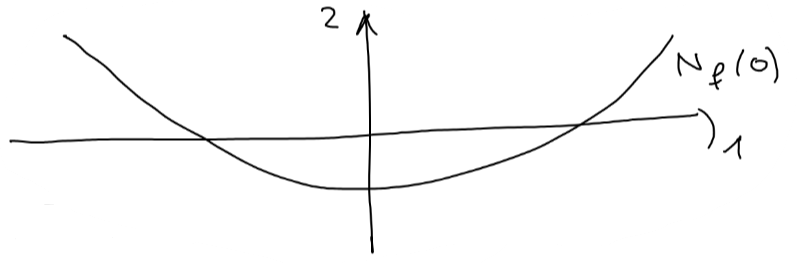
\includegraphics[width=0.5\linewidth]{figures/implizite_funktion_beispiel_kein_eingeschraenkter_definitionsbereich}
      \label{fig:implizite_funktion_beispiel_kein_eingeschraenkter_definitionsbereich}
    \end{figure}
    \item \( f(x,y)=3x-y^2+1 \) auf \( \reals^2 \). \( \totalderivative-{f}(a,b)=\begin{pNiceMatrix} 3 & -2b \end{pNiceMatrix} \). \ref{satz_von_der_impliziten_funktion} \timplies Zu \( b\neq 0 \) gibt es \( g\maps I\to \reals \). \( b>0 \): \( g(x)=+\sqrt{3x+1} \), \( x>-\frac{1}{3} \). \( b<0 \): \( g(x)=-\sqrt{3x+1} \).
    \begin{figure}[H]
      \centering
      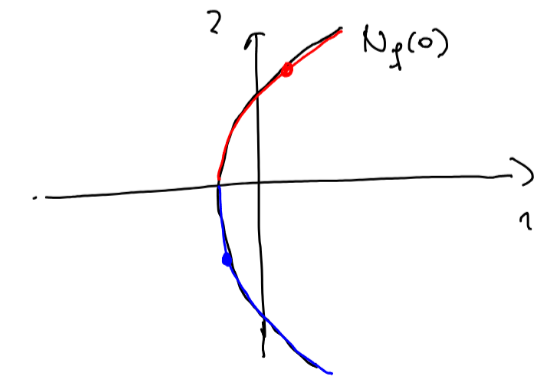
\includegraphics[width=0.5\linewidth]{figures/implizite_funktion_beispiel_eingeschraenkter_definitionsbereich}
      \caption*{\( f(x,g(x))=0 \)}
      \label{fig:implizite_funktion_beispiel_eingeschraenkter_definitionsbereich}
    \end{figure}
  \end{enumerate}
\end{beispiele*}
\begin{proof}[Beweis von \thref{satz_von_der_impliziten_funktion}]
  \begin{proofenumerate}[label=\rechtsklammer{\arabic*}]
    Setze \( B\definedas D_2f(a,b)\) und definiere eine Abbildung \( h\maps U_1\times U_2\to \reals^m \) vermöge
    \begin{equation*}
      h(x,y)=y-b-\inverse{B} f(x,y).
    \end{equation*}
    Dann gilt 
    \begin{equation*}
      D_2 h(x,y)=\mathds{1}-\inverse{B} D_2 f(x,y).
    \end{equation*}
    \timplies \( D_2 h(a,b)=0 \) \timplies (da alle Ableitungen stetig sind) \texists \( W_1\subset U_1 \), \( W_2\subset U_2 \) offene Umgebungen von \( a \) \bzw \( b \) \sd
    \begin{equation*}
    \norm{D_2 h(x,y)}\leq \frac{1}{2}\quad \forall x\in W_1,\logicspace y\in W_2\tag{\(*\)}.\label{satz_von_der_impliziten_funktion:beweis:h:ableitungsnorm_bschraenkt}
    \end{equation*}
    Wähle \( r>0 \) \sd \( V_2\definedas B_r^{\norm{\cdot}}(b)\subset W_2 \). Es ist \( h(a,b)=0 \) \timplies (da \( h \) differenzierbar ist und somit auch stetig) \texists offene Umgebung \( V_1\subset W_1 \) von \( a \) \sd 
    \begin{equation*}
      \varepsilon\definedas \sup_{x\in V_1}\norm{h(x,b)}<\frac{r}{2} \tag{\( ** \)}\label{satz_von_der_impliziten_funktion:beweis:h:norm_beschraenkt}
    \end{equation*}
    (auf einem Kompaktum \( \subset W_1 \) um \( a \) ist \( x\mapsto h(x,b) \) beschränkt und wird auf einem hinreichend kleinen Kompaktum beliebig klein. Um \( V_1 \) offen zu erhalten, nehmen wir das Innere eines solchen Kompaktums).
    \item Wir zeigen jetzt: Zu jedem \( x\in V_1 \) gibt es höchstens ein \( y\in V_2 \) \sd \( f(x,y)=0 \) also \sd \( h(x,y)=y-b \).
    
    Sei also \( x\in V_1 \) und seien \( y_1 \) und \( y_2 \) \sd \( h(x,y_1)=y_1-b \) und \( h(x,y_2)=y_2-b \).
    \begin{align*}
      \implies &y_1-y_2=h(x,y_1)-h(x,y_2)\\
      \underset{\mathclap{\text{MWS und \eqref{satz_von_der_impliziten_funktion:beweis:h:ableitungsnorm_bschraenkt}}}}{\implies}&\norm{y_1-y_2}\begin{aligned}[t]
        &=\norm{h(x,y_1)-h(x,y_2)}\\
        &\explain{\text{\( \zeta \) auf der Verbindungsstrecke zw.\ \( y_1 \) und \( y_2 \) (liegt in \( V_2=B_r(b) \))}}{=}\norm{D_2 h(x,\zeta)}\matrixmult\norm{y_1-y_2}\\
        &\leq \frac{1}{2}\norm{y_1-y_2}
      \end{aligned}\\
      \implies &\norm{y_1-y_2}=0 \implies y_1=y_2.
    \end{align*}
    \item Wir zeigen nun die Existent einer Funktion \( g \) wie im Satz behauptet. Setze dazu \( g_0(x)=b \) und definiere rekursiv für \( x\in V_1 \):
    \begin{equation*}
      g_{j+1}(x)\definedas b+h(x,g_j(x)).
    \end{equation*}
    \begin{proofenumerate}[label=\rechtsklammer{\alph*}]
      \item Es gilt
      \begin{equation*}
        \norm{g_{j+1}-g_j}_{\infty, V_1}\leq 2^{-j}\explain{\text{aus \eqref{satz_von_der_impliziten_funktion:beweis:h:norm_beschraenkt}}}{\varepsilon}.
      \end{equation*}
      Induktionsanfang: 
      \begin{equation*}
        \norm{g_1-g_0}_{\infty,V_1}=\norm{h(x,b)}_{\infty, V_1}=\varepsilon.
      \end{equation*}
      Induktionsschritt: Sei die Behauptung für \( i\leq n \) bewiesen. 
      \begin{align*}
        &g_{n+2}(x)-g_{n+1}(x)=h(x,g_{n+1}(x))-h(x,g_n(x)).\\
        \underset{\mathclap{\text{MWS und \eqref{satz_von_der_impliziten_funktion:beweis:h:ableitungsnorm_bschraenkt}}}}{\implies}&\norm{g_{n+2}-g_{n+1}}_{\infty,V_1}\leq \frac{1}{2}\norm{g_{n+1}-g_n}_{\infty,V_1}.
      \end{align*}
      \begin{bemerkung*}
        Der MWS darf tatsächlich angewendet werden. \( g_{n+1}(x), g_n(x) \) und somit auch die Verbindungsstrecke zwischen ihnen liegen in \( V_2 \), denn nach Induktionsvoraussetzung gilt für alle \( j\leq n \)
        \begin{equation*}
          \norm{g_{j+1}-b}_{\infty,V_1}\leq \sum_{i=0}^{j}\norm{g_{i+1}-g_i}\leq 2\varepsilon<r
        \end{equation*}
        (da \( g_{j+1}-b=\sum_{i=0}^{j}(g_{i+1}-g_i) \) ist). Somit darf der MWS auf
        \begin{equation*}
          h(x,g_{n+1}(x))-h(x,g_n(x))
        \end{equation*}
        angewendet werden.
      \end{bemerkung*}
      \item Es folgt \( \norm{g_n-b}_{\infty, V_1}<r \) und somit \( g_n(V_1)\subset V_2 \). Denn
      \begin{align*}
        &g_n=\sum_{j=0}^{n-1} (g_{j+1}-g_j)+b\quad (\text{Teleskopsumme})
        \implies &\norm{g_n-b}_{\infty,V_1}\leq \sum_{j=0}^{n-1}2^{-j}\varepsilon \explain{\text{geom.\ Reihe}}{\leq}2\varepsilon<r.
      \end{align*}
      \item Zudem gilt: \( \norm{\sum_{j=0}^{\infty}(g_{j+1}-g_j)}_{\infty,V_1} \) hat die Majorante \( \sum_{j=0}^{\infty}2^{-j}\varepsilon \). \timplies Die Reihe konvergiert gleichmäßig auf \( V_1 \) \timplies (Diff \Romannum{1})
      \begin{equation*}
        g\definedas \lim_{n \goesto \infty} g_n=\sum_{j=0}^{\infty}(g_{j+1}-g_j)+b
      \end{equation*}
      ist stetig auf \( V_1 \) und
      \begin{equation*}
        \norm{g-b}_{\infty,V_1}\leq 2\varepsilon<r,
      \end{equation*}
      also \( g(V_1)\subset V_2 \).
    \end{proofenumerate}
    Aus der Definition folgt durch Grenzübergang auf beiden Seiten (\( h \) ist stetig)
    \begin{equation*}
      g(x)=b+h(x,g(x))\quad \forall x\in V_1,
    \end{equation*}
    also \( g(x)=g(x)-\inverse{B}f(x,g(x)) \), also
    \begin{equation*}
      f(x,g(x))=0\quad \forall x\in V_1.
    \end{equation*}
  \end{proofenumerate}
\end{proof}
\begin{folgerung}\label{satz_von_der_impliziten_funktion:hoehenlinie_folgerung}
  Sei \( f\maps U\to \reals \), \( U\subset \reals^2 \) offen, stetig differenzierbar und sei \( \ointerval{a}{b}\in U \), \( f(a,b)=c \) und \( \grad-{f(a,b)}\neq 0 \). Dann kann man ein Stück der Höhenlinie \( N_f(c) \) als Graph einer FUnktion beschreiben. Denn sei \( \partial_2 f(a,b)\neq 0 \), \thref{satz_von_der_impliziten_funktion},  angewandt auf \( \tilde{f(x,y)}=f(x,y)-c \), impliziert:

  \texists Intervalle \( I_1,I_2 \), \( a\in I_1 \), \( b\in I_2 \), \( I_1\times I_2\subset U \) und eine stetig differenzierbare Funktion (Bemerkung \ref{implizite_funktion_auf_umgebung_stetig_differenzierbar}) \( g\maps I_1\to \reals \), mit \( g(I_1)\subset I_2 \) und
  \begin{multline*}
    N_f(c)\cap I_1\times I_2=\Set{(x,y)\in I_1\times I_2|\tilde{f}(x,y)=0}=\Set{(x,g(x))|x\in I_1}=\Gamma_g.
  \end{multline*}
  Dito für den Fall, dass \( \partial_1 f(a,b)\neq 0 \) ist (mit vertauschten Rollen für \( x, y \)), also
  \begin{equation*}
    N_f(c)\cap I_1\times I_2=\Set{(g(x),x)|x\in I_2}.
  \end{equation*}
\end{folgerung}
